\newpage\pagestyle{main}

\chapter{Valutazione Sperimentale e Analisi delle Performance}\label{chap:fifth}

\inlineminitoc

% ─────────────────────────────────────────────────────────────────────────────
\section{Setup dei test e Metodologia}

La valutazione di un sistema di \textit{Conversational AI} basato su RAG distribuito richiede un'analisi multidimensionale. Non è sufficiente che la risposta sia corretta, essa deve essere fornita in un tempo compatibile con le dinamiche della conversazione umana. In letteratura, il limite superiore per una conversazione percepita come fluida e naturale è identificato intorno ai 2 secondi di latenza complessiva \cite{latency_eca}. Superare questa soglia interrompe la fluidità del dialogo e può portare a una diminuzione dell'esperienza utente indipendentemente dalla qualità del contenuto della risposta.

Per questo motivo, la sperimentazione si è concentrata sulla misurazione della della query, costruendo un protocollo di test progettato per isolare il contributo specifico dell'architettura distribuita rispetto a un approccio monolitico. Le variabili non pertinenti all'oggetto di indagine, come la latenza di rete verso ElevenLabs o il tempo di riproduzione audio in Unreal Engine, sono state tenute fuori dall'analisi, poiché non risentono delle ottimizzazioni introdotte dalla logica di sharding.

% ─────────────────────────────────────────────────────────────────────────────
\subsection{Dataset e Popolamento del Grafo}

Per i test è stata utilizzata una Knowledge Base tecnica composta da manuali operativi in formato PDF riguardanti il dominio dell'epilessia. La scelta di un dominio medico specialistico non è casuale, poiché le basi di conoscenza in ambito clinico presentano caratteristiche strutturali che stressano in modo particolarmente efficace il sistema, tra cui un'alta densità di relazioni inter-documento, una terminologia fortemente specializzata che sfida i modelli di embedding, e una struttura gerarchica dei contenuti che si presta naturalmente alla rappresentazione a grafo.

I documenti sono stati processati, frammentati in paragrafi e inseriti nel database Neo4j remoto seguendo lo schema descritto nel Capitolo \ref{chap:second}. Durante la fase di indicizzazione, per ogni nodo \texttt{PARAGRAPH} sono stati generati automaticamente tramite l'LLM i nodi \texttt{QUESTION} e \texttt{STATEMENT} associati, e per ognuno di essi è stato calcolato il vettore di embedding tramite \textbf{Embedding-Gemma} \cite{embedding_gemma_2025} in esecuzione locale via Ollama \cite{ollama}.

Il grafo finale conta circa \textbf{20.000 nodi interconnessi}, tra cui circa \textbf{600 nodi di tipo \texttt{PARAGRAPH}}. Questa dimensione, pur essendo contenuta rispetto a una base di conoscenza clinica reale, è sufficiente per rilevare differenze di prestazione tra le due architetture a confronto. È ragionevole attendersi che i benefici dello sharding siano ancora più pronunciati al crescere della dimensione del dataset, poiché la latenza di accesso al Remote scala in modo non lineare con la dimensione dell'indice vettoriale.

% ─────────────────────────────────────────────────────────────────────────────
\subsection{Configurazione Hardware}

I test sono stati condotti in un ambiente controllato per isolare il più possibile l'impatto dell'architettura software da quello dell'hardware sottostante. La configurazione utilizzata è la seguente:

\begin{itemize}
    \item \textbf{Processore}: AMD RYZEN 5 7600, 3.8 GHz (6 core, 12 thread).
    \item \textbf{Memoria RAM}: 32 GB DDR5 @6400 MHz.
    \item \textbf{GPU}: NVIDIA GeForce RTX 4070 SUPER, 12 GB VRAM.
\end{itemize}

La GPU si è rivelata fondamentale per garantire tempi di risposta accettabili durante l'elaborazione locale. I pesi di \textbf{Llama 3.2} (3B parametri) e del modello \textbf{Embedding-Gemma} sono stati caricati interamente sulla memoria video tramite Ollama \cite{ollama}, evitando così il continuo trasferimento dei dati tra RAM e disco durante l'elaborazione. Senza una GPU dedicata, entrambi i modelli sarebbero stati costretti a funzionare sulla sola CPU, con tempi di risposta lunghi. L'uso di hardware consumer dimostra tuttavia che l'architettura proposta non richiede ambienti server specializzati, rendendo molto più accessibile l'adozione della soluzione.

% ─────────────────────────────────────────────────────────────────────────────
\section{Metriche di Valutazione}

Per quantificare le prestazioni del sistema è stata adottata come metrica principale la latenza \textit{end-to-end}, definita come il tempo totale (\textit{Round Trip Time}, RTT) intercorrente tra il momento in cui l'embedding della domanda è disponibile per la query e il momento in cui il sistema restituisce i documenti necessari per la generazione della risposta. Questa definizione esclude deliberatamente il tempo dei modelli di generazione e del componente Unreal, poiché questi contributi sono indipendenti dalla scelta dell'architettura di recupero e avrebbero introdotto varianza non pertinente all'analisi.

La latenza end-to-end così definita misura specificamente il tempo necessario al sistema per recuperare e mettere a disposizione il contesto per la risposta. Nel caso dell'architettura monolitica, questa include esclusivamente il tempo di recupero remoto, cioè la ricerca vettoriale sul database cloud, la navigazione del grafo per l'espansione contestuale, e il trasferimento dei risultati. Nel caso dell'architettura distribuita, il tempo misurato include sia il tempo di recupero remoto sia il tempo di sincronizzazione con lo Shard locale. È proprio questo secondo termine che rappresenta il maggiore differenziale architetturale e il fulcro dell'analisi. Nelle query successive, quando il contesto è già presente nello Shard, questo tempo tende a ridursi, riducendo il RTT complessivo.

Non è stata presa in considerazione la qualità semantica delle risposte come metrica di valutazione in questa fase. Per costruzione, il contenuto del contesto fornito all'LLM è identico nei due sistemi a confronto per ogni domanda. La differenza tra le due architetture riguarda esclusivamente il tempo necessario a recuperare quel contesto, e non la sua qualità.

% ─────────────────────────────────────────────────────────────────────────────
\section{Analisi Comparativa: Monolitico vs. Distribuito}

L'esperimento principale consiste nel confrontare il comportamento del sistema Monolitico con quello del sistema Distribuito. Le due configurazioni sono identiche in ogni altro aspetto. Hanno stesso modello LLM, stesso modello di embedding, stesso schema del grafo, stesso dataset.

% ─────────────────────────────────────────────────────────────────────────────
\subsection{Protocollo di Test e Scelta delle Query}

Per la valutazione sono state formulate cinque query progressive, selezionate in modo da coprire scenari rappresentativi del ciclo di vita della cache durante una sessione conversazionale reale. Le query seguono una progressione semantica che rispecchia il modo in cui un utente potrebbe esplorare un argomento medico in modo naturale, partendo da un aspetto specifico e allargando gradualmente il campo della discussione:

\begin{enumerate}
    \item \textit{"In quale condizione potrebbero essere associate le irregolarità mestruali all'epilessia?"}\\
          È la prima domanda della sessione, quando lo Shard è ancora vuoto. Il sistema deve andare al Remote e popolare la cache, è il classico caso di \textbf{Cold Start}.

    \item \textit{"Gli effetti dei farmaci antiepilettici sugli ormoni riproduttivi possono essere diretti o indiretti?"}\\
          È molto vicina alla prima, quindi parte del contesto è già in cache. Qui ci si aspetta i primi \textbf{cache hit}.

    \item \textit{"Ci sono fattori psicologici associati all'epilessia che possono influire sulla decisione di diventare genitori?"}\\
          Qui il tema cambia un po', ma resta coerente. Il sistema deve aggiungere nuovi dati senza perdere quelli già acquisiti, è un buon caso di \textbf{espansione del contesto}.

    \item \textit{"Come gestisco le convulsioni dei neonati?"}\\
          È una domanda più distante dalle precedenti, quindi lo Shard aiuta meno. La latenza si avvicina a quella del sistema monolitico.

    \item \textit{"Cos'è l'epilessia?"}\\
          È una domanda molto generica, quindi richiede molti nodi. Allo stesso tempo, può sfruttare bene ciò che lo Shard ha già in memoria.
\end{enumerate}

% ─────────────────────────────────────────────────────────────────────────────
\subsection{Risultati e Analisi per Domanda}

I tempi di risposta misurati nelle due configurazioni sono riportati di seguito.

\begin{table}[h]
    \centering
    \begin{tabular}{|l|c|c|c|}
        \hline
        \textbf{Domanda di test} & \textbf{Senza Sharding (ms)} & \textbf{Con Sharding (ms)} & \textbf{Delta (\%)} \\ \hline
        Domanda 1 (Cold Start)   & 187                          & 216                        & +13.4\%             \\ \hline
        Domanda 2 (Correlata)    & 207                          & 174                        & -15.9\%             \\ \hline
        Domanda 3 (Espansione)   & 321                          & 217                        & -32.4\%             \\ \hline
        Domanda 4 (Nuovo arg.)   & 205                          & 177                        & -13.7\%             \\ \hline
        Domanda 5 (Generica)     & 240                          & 191                        & -20.4\%             \\ \hline
    \end{tabular}
    \caption{Confronto dei tempi tra sistema monolitico e sistema distribuito.}
    \label{tab:performance_results}
\end{table}

\begin{figure}[h]
    \centering
    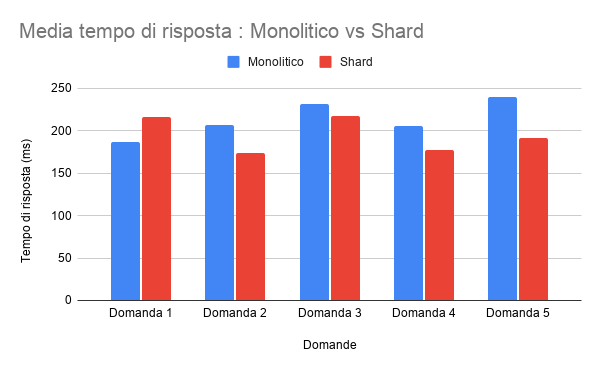
\includegraphics[width=1\textwidth]{_figures/latency_chart.png}
    \caption{Confronto della latenza di recupero tra sistema monolitico e sistema distribuito.}
    \label{fig:latency_chart}
\end{figure}

\newpage

L'analisi della Tabella~\ref{tab:performance_results} e del Grafico~\ref{fig:latency_chart} evidenzia con chiarezza il comportamento atteso dell'architettura distribuita e ne conferma l'efficacia a partire dalla seconda interrogazione della sessione.

\begin{itemize}
    \item \textbf{Cold Start (+13.4\%).} Come atteso, la cache è inizialmente vuota e il sistema deve ricorrere al Remote, pagando il costo della sincronizzazione locale tra le operzioni di upsert dei nodi, inizializzazione di \texttt{hit\_count} e \texttt{last\_accessed}, creazione delle relazioni \texttt{HAS\_PARAGRAPH}. L'overhead di 29 ms è un investimento che si ripaga già alla query successiva.

    \item \textbf{Cache Hit (-15.9\%).} Quando la domanda è semanticamente correlata alla precedente, lo Shard già popolato offre un vantaggio immediato. I paragrafi vengono recuperati localmente, risparmiando 33 ms e compensando completamente il costo iniziale.

    \item \textbf{Espansione del Contesto (-32.4\%).} La domanda sulla psicologia e genitorialità beneficia del context windowing . Il guadagno di 104 ms dimostra che non solo i paragrafi direttamente cercati rimangono in cache, ma anche i loro vicini strutturali, con effetti positivi sulle sessioni a lungo termine.

          \newpage

    \item \textbf{Nuovo Argomento (-13.7\%).} Con l'argomento sulle crisi neonatali, il vantaggio diminuisce poiché molti nodi non sono ancora in cache. Il sistema deve accedere al Remote, ma conserva comunque un risparmio di 28 ms grazie ai contenuti acquisiti nelle query precedenti e ancora rilevanti.

    \item \textbf{Query Generica ad Alto Richiamo (-20.4\%).} La domanda sulla definizione generale dell'epilessia richiede molti nodi, ma ne trova una frazione significativa già acquisiti. Il risparmio di 49 ms testimonia come una sessione ben strutturata costruisca progressivamente una cache che copre il dominio in modo sempre più ampio.
\end{itemize}

% ─────────────────────────────────────────────────────────────────────────────
\subsection{Considerazioni sul Bilanciamento del Cold Start}

Un aspetto rilevante dei risultati è la velocità con cui il costo del Cold Start viene ammortizzato. Il vantaggio cumulativo delle quattro query successive alla prima ammonta a $33 + 104 + 28 + 49 = 214$ ms, mentre il costo iniziale è stato di soli 29 ms. Il bilancio netto dell'intera sessione di cinque domande è quindi un risparmio cumulativo di 185 ms, già con un dataset di dimensioni modeste e sole cinque domande. In sessioni più lunghe e con basi di conoscenza più estese il vantaggio cumulativo è destinato ad aumentare ulteriormente.

Vale la pena osservare, inoltre, che il costo del Cold Start potrebbe essere ridotto con strategie di pre-warming dello Shard, dove all'avvio di una sessione, il sistema potrebbe eseguire preventivamente una serie di query predefinite sui topic più frequentemente richiesti dagli utenti, pre-popolando lo shard prima che l'utente inizi a interagire.

% ─────────────────────────────────────────────────────────────────────────────
\section{Efficacia della logica di Eviction LFU}

Uno degli aspetti più delicati dell'architettura distribuita è mantenere stabile lo Shard locale quando la conversazione si prolunga. Senza un controllo sulla dimensione della cache, infatti, lo Shard continuerebbe a crescere fino a occupare troppa memoria o a rallentare le prestazioni, perché il grafo diventerebbe sempre più grande e costoso da gestire.

Per verificare quanto la politica di gestione della memoria sia davvero robusta, lo Shard locale è stato monitorato durante una sessione intensa di \textbf{50 domande consecutive}, che ha coperto l'intero dominio della Knowledge Base relativa all'epilessia.

% ─────────────────────────────────────────────────────────────────────────────
\subsection{Occupazione di Memoria e Stabilità}

Nel corso delle 50 domande, l'occupazione dello Shard mostra un andamento progressivo e facilmente leggibile. All'inizio, ogni nuova richiesta introduce nodi che non erano ancora presenti in cache, quindi il numero di \texttt{PARAGRAPH} cresce rapidamente mentre il sistema costruisce la propria memoria operativa sul dominio.

Con il procedere della sessione, il numero di nodi si avvicina alla soglia di 30. Le query continuano ad ampliare il contenuto dello Shard, ma l'algoritmo di eviction interviene sui nodi meno rilevanti, mantenendo la cache entro il limite previsto. Questo comportamento conferma che la macro-query Cypher gestisce correttamente l'inserimento e la rimozione dei dati in modo coerente con le operazioni di scrittura.

Quando la sessione entra nella sua parte più stabile, lo Shard tende a mantenere i nodi effettivamente utili. Quelli consultati più spesso restano disponibili in cache con un \texttt{hit\_count} crescente, mentre i nodi meno usati vengono progressivamente sostituiti da nuovi contenuti. In questo modo, la cache finisce per rispecchiare in modo naturale gli argomenti affrontati durante la conversazione.

\begin{figure}[htbp]
    \centering
    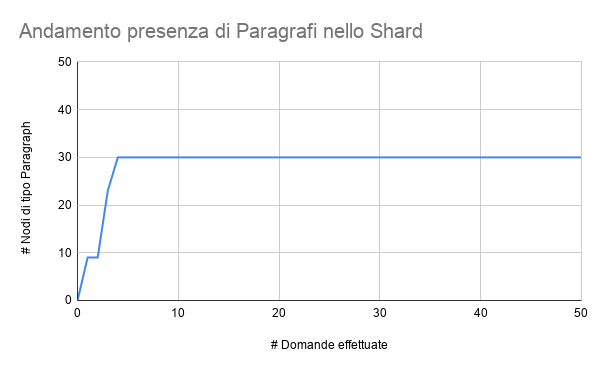
\includegraphics[width=1\textwidth]{_figures/sharding_saturation.png}
    \caption{Andamento del numero di nodi nello Shard locale durante una sessione intensiva di 50 domande.}
    \label{fig:saturation}
\end{figure}

La politica \textbf{Least Frequently Used (LFU)}, basata sui parametri \texttt{hit\_count} e \texttt{last\_accessed}, si è dimostrata una scelta solida per il tipo di conversazione osservato nei test. Rispetto a una politica LRU (\textit{Least Recently Used}), che eliminerebbe semplicemente i nodi non usati nell'ultima query, la LFU mantiene invece i contenuti che vengono richiamati più spesso nel tempo. In pratica, questo significa che i nodi davvero importanti restano disponibili anche se l'utente, per qualche domanda, si sposta temporaneamente su un argomento vicino ma diverso. È un comportamento più naturale e più coerente con una sessione medica, dove si tende spesso a tornare sugli stessi concetti per fare ulteriori approfondimenti.

Un altro aspetto positivo emerso riguarda l'assenza di \textit{cache thrashing}. Nei sistemi con una soglia di memoria troppo rigida, infatti, può capitare che gli stessi nodi vengano rimossi e reinseriti di continuo, con un impatto evidente sulle prestazioni. Nel corso della sessione di 50 domande questo problema non si è presentato. Il limite di 30 nodi ha permesso di conservare in cache il contesto davvero utile, senza generare oscillazioni anomale nella composizione dello Shard. Per il dataset e per il dominio considerati, questa soglia si è quindi rivelata adeguata.

% ─────────────────────────────────────────────────────────────────────────────
\section{Analisi della Query Plan Cache}

Oltre al vantaggio dello sharding sulla latenza, c'è un secondo aspetto che contribuisce all'efficienza complessiva del sistema, ovvero l'uso di query parametrizzate \cite{neo4j_benchmarking}. Questa scelta di design lavora in parallelo rispetto allo sharding e lo rende ancora più efficace.

Il principio è semplice, Neo4j dispone di una \textit{Execution Plan Cache} che memorizza come eseguire una query. Quando una query parametrizzata viene lanciata per la prima volta, il database analizza la struttura della domanda, calcola il modo migliore di rispondere e conserva questo piano in memoria. Le volte successive, se la struttura rimane la stessa e cambiano solo i dati, il database recupera il piano già pronto e lo applica direttamente, saltando tutta la fase di calcolo iniziale.

Questo aiuta particolarmente nel nostro sistema per due motivi principali. Innanzitutto, la macro-query che sincronizza lo Shard locale è piuttosto complessa, dato che contiene ricerche vettoriali, navigazione del grafo, logica condizionale e operazioni di scrittura. Calcolare come eseguire questa query ogni volta comporterebbe un costo computazionale che si accumulerebbe rapidamente. Inoltre, durante una conversazione, l'utente fa domande diverse, ma il motore usa sempre la stessa macro-query, solo il vettore della domanda cambia ad ogni turno. Grazie al caching, dalla seconda domanda in poi, il sistema salta interamente questa fase di preparazione.

Monitorando i log di Neo4j durante i test, è stato verificato che il piano di esecuzione viene calcolato una sola volta all'inizio della conversazione e poi riutilizzato per tutte le domande successive. Questo comportamento è esattamente quello che ci aspettiamo dalla documentazione ufficiale di Neo4j \cite{neo4j_benchmarking} e rappresenta una pratica consolidata che il nostro sistema implementa sistematicamente mediante l'uso esclusivo di parametri nelle query Cypher.

Sharding e query plan cache si completano a vicenda. Lo sharding riduce quante volte serve accedere al database remoto e quanto tempo il network richiede, mentre il query plan cache riduce il tempo che il database impiega a preparare l'esecuzione, sia sul Remote che sullo Shard locale. Operano su livelli diversi del tempo totale di risposta, e i loro vantaggi si sommano naturalmente senza ostacolarsi.

\newpage

% ─────────────────────────────────────────────────────────────────────────────
\section{Interpretazione dei risultati}

I dati raccolti durante la campagna sperimentale mostrano che l'architettura proposta funziona bene, ma ha anche alcuni limiti da tenere presenti.

Il confronto tra sistema monolitico e distribuito conferma che, anche con un dataset moderato di circa 600 nodi \texttt{PARAGRAPH}, l'accesso ripetuto a un database remoto introduce una latenza poco prevedibile e può rallentare la conversazione. Nel sistema monolitico, infatti, tutto dipende dalla rete verso il cloud. Con il sistema distribuito, invece, dalla seconda query in poi il recupero passa in locale e diventa più stabile \cite{kleppmann2017}. In un sistema di Conversational AI questo è importante quanto il tempo medio di risposta.

Il beneficio aumenta con la complessità del dominio. Nel nostro caso i risparmi sono di alcune decine di millisecondi per query perché il dataset è piccolo e le domande sono abbastanza semplici. In scenari reali, con basi di conoscenza più grandi, il costo di accesso al Remote crescerebbe per l'indice vettoriale, la navigazione del grafo e il traffico di rete. L'architettura distribuita serve proprio a ridurre questi effetti e a mantenere prestazioni più costanti \cite{rag_performance_2023}.

Anche la logica di eviction ha dato risultati positivi. La politica LFU mantiene in cache i nodi davvero usati e rimuove quelli meno utili, così il contesto resta coerente durante tutta la sessione. Nei test, la qualità delle risposte è rimasta stabile per 50 domande, e la soglia di 30 nodi si è rivelata adeguata.

Resta però una limitazione importante, ovvero che la valutazione riguarda un solo dominio, un numero ridotto di query e nessuno scenario concorrente. Inoltre, non sono state usate metriche automatiche come ROUGE o BERTScore per misurare in modo sistematico la qualità semantica. I risultati sono quindi solidi sul piano della latenza, ma non esauriscono la valutazione complessiva del sistema.